%%%%%%%%%%%%%%%%%%%%%%%%%%%%%%%%%%%%%%%%%%%%%%%%%%%%%%%%%%%%%%%

% Document Header %

% Importing Libraries %
\documentclass[12pt, a4paper,openany]{article}
\usepackage{caption}
\usepackage{listings}
\usepackage{titlesec}
\usepackage{subcaption}
\usepackage[utf8]{inputenc}
\usepackage{amsmath} 
\usepackage[colorlinks=true, urlcolor=blue, linkcolor=blue]{hyperref}
\usepackage{graphicx} 
\usepackage[a4paper, total={6in, 9in}]{geometry}
\usepackage{titling}

\usepackage{tikz}
\usetikzlibrary{shapes.geometric, arrows}
\usetikzlibrary{positioning}
\usetikzlibrary{calc}
% Defining Defaults %
\usepackage[table,xcdraw]{xcolor}
\graphicspath{{Images/}}
\titlespacing*{\section}{0pt}{-1pt}{1.5\baselineskip}
\titlespacing*{\subsection}{0pt}{*1}{1.0\baselineskip}
% Defining tikzstyle for Flow Charts %
\tikzstyle{ghost} = [rectangle, 
minimum width=1.5cm, 
minimum height=1cm, 
text centered, 
text width=1cm, 
draw=black!0 
]
\tikzstyle{startstop} = [rectangle, rounded corners, 
minimum width=3cm, 
minimum height=1cm,
text centered, 
text width = 5cm,
draw=black, 
fill=red!20]

\tikzstyle{startstop_o} = [rectangle, rounded corners, 
minimum width=3cm, 
minimum height=1cm,
text centered, 
text width = 5cm,
draw=black, 
fill=orange!20]

\tikzstyle{startstop_c} = [rectangle, rounded corners, 
minimum width=3cm, 
minimum height=1cm,
text centered, 
text width = 5cm,
draw=black, 
fill=green!20]

\tikzstyle{startstop_cy} = [rectangle, rounded corners, 
minimum width=3cm, 
minimum height=1cm,
text centered, 
text width = 5cm,
draw=black, 
fill=cyan!20]

\tikzstyle{startstop_y} = [rectangle, rounded corners, 
minimum width=3cm, 
minimum height=1cm,
text centered, 
text width = 5cm,
draw=black, 
fill=yellow!20]


\tikzstyle{startstop_w} = [rectangle, rounded corners, 
minimum width=3cm, 
minimum height=1cm,
text centered, 
text width = 6cm,
draw=black, 
fill=red!20]

\tikzstyle{startstop_wg} = [rectangle, rounded corners, 
minimum width=3cm, 
minimum height=1cm,
text centered, 
text width = 6cm,
draw=black, 
fill=green!20]

\tikzstyle{startstop_wb} = [rectangle, rounded corners, 
minimum width=3cm, 
minimum height=1cm,
text centered, 
text width = 6cm,
draw=black, 
fill=blue!20]

\tikzstyle{startstop_wr} = [rectangle, rounded corners, 
minimum width=3cm, 
minimum height=1cm,
text centered, 
text width = 6cm,
draw=black, 
fill=red!20]

\tikzstyle{process} = [rectangle, 
minimum width=3cm, 
minimum height=1cm, 
text centered, 
text width=5cm, 
draw=black, 
fill=orange!30]

\tikzstyle{process_c} = [rectangle, 
minimum width=3cm, 
minimum height=1cm, 
text centered, 
text width=5cm, 
draw=black, 
fill=cyan!30]


\tikzstyle{process_small} = [rectangle, 
minimum width=3cm, 
minimum height=1cm, 
text centered, 
text width=4cm, 
draw=black, 
fill=orange!30]

\tikzstyle{process_smallc} = [rectangle, 
minimum width=3cm, 
minimum height=1cm, 
text centered, 
text width=4cm, 
draw=black, 
fill=cyan!30]

\tikzstyle{process_wide} = [rectangle, 
minimum width=3cm, 
minimum height=1cm, 
text centered, 
text width=6cm, 
draw=black, 
fill=orange!30]

\tikzstyle{process_widec} = [rectangle, 
minimum width=3cm, 
minimum height=1cm, 
text centered, 
text width=6cm, 
draw=black, 
fill=cyan!30]

\tikzstyle{process_uwide} = [rectangle, 
minimum width=3cm, 
minimum height=1cm, 
text centered, 
text width=8cm, 
draw=black, 
fill=orange!30]

\tikzstyle{process_uwidec} = [rectangle, 
minimum width=3cm, 
minimum height=1cm, 
text centered, 
text width=8cm, 
draw=black, 
fill=cyan!30]

\usepackage{xcolor}
\definecolor{codegreen}{rgb}{0,0.6,0}
\definecolor{codegray}{rgb}{0.5,0.5,0.5}
\definecolor{codepurple}{rgb}{0.58,0,0.82}
\definecolor{backcolour}{rgb}{0.95,0.95,0.92}
\tikzstyle{line} = [draw,-latex]



% Defining Title Sequence %
\title{\vspace{-3cm} \makebox[\textwidth][c]{COL215 SW Assignment 1 - Gate Packing}}
\author{Submission By :\\ \hspace{0.5cm} \textbf{Yash Rawat} \hspace{1cm} \textbf{Priyanshi Gupta}\\ \textbf{2023CS50334} \hspace{1.3cm} \textbf{2023CS10106} \\ \\ Department of Computer Science and Engineering \\ Indian Institute of Technology, Delhi}
\date{\today}
% Ending Document Header %

%%%%%%%%%%%%%%%%%%%%%%%%%%%%%%%%%%%%%%%%%%%%%%%%%%%%%%%%%%%%%%%
% Starting document Page 1%
%%%%%%%%%%%%%%%%%%%%%%%%%%%%%%%%%%%%%%%%%%%%%%%%%%%%%%%%%%%%%%%
\begin{document} 
\lstdefinestyle{mystyle}{
  backgroundcolor=\color{backcolour}, commentstyle=\color{codegreen},
  keywordstyle=\color{magenta},
  numberstyle=\tiny\color{codegray},
  stringstyle=\color{codepurple},
  basicstyle=\ttfamily\footnotesize,
  breakatwhitespace=false,         
  breaklines=true,                 
  captionpos=b,                    
  keepspaces=true,                 
  numbers=left,                    
  numbersep=5pt,                  
  showspaces=false,                
  showstringspaces=false,
  showtabs=false,                  
  tabsize=1
}
\lstset{style=mystyle}


\maketitle

% B_Roll For Project in Minipage Env %
\begin{figure}[ht]
\centering
  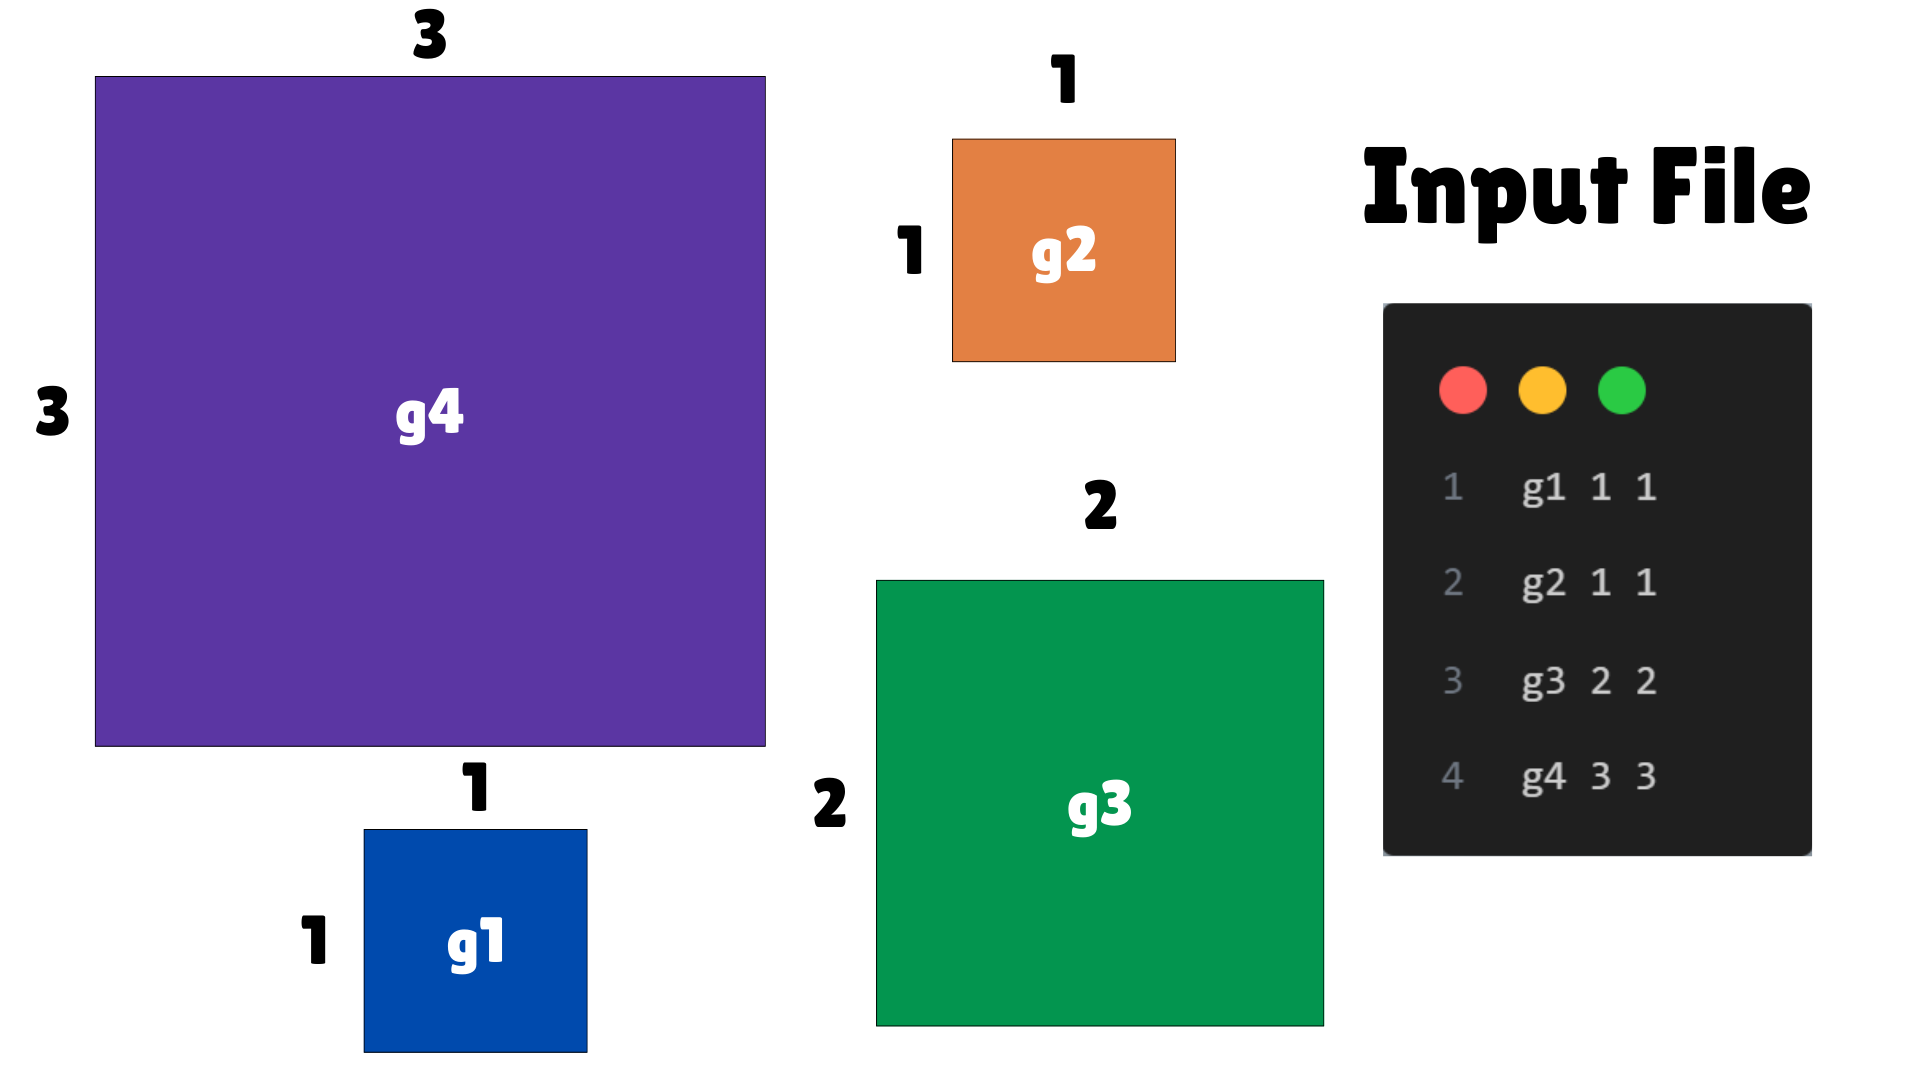
\includegraphics[width=0.8\linewidth]{BRoll/tc1_rep}
  % \captionof{figure}{A figure}
  \label{fig:basys_b}
\end{figure}
\begin{figure}[ht]
  \centering
  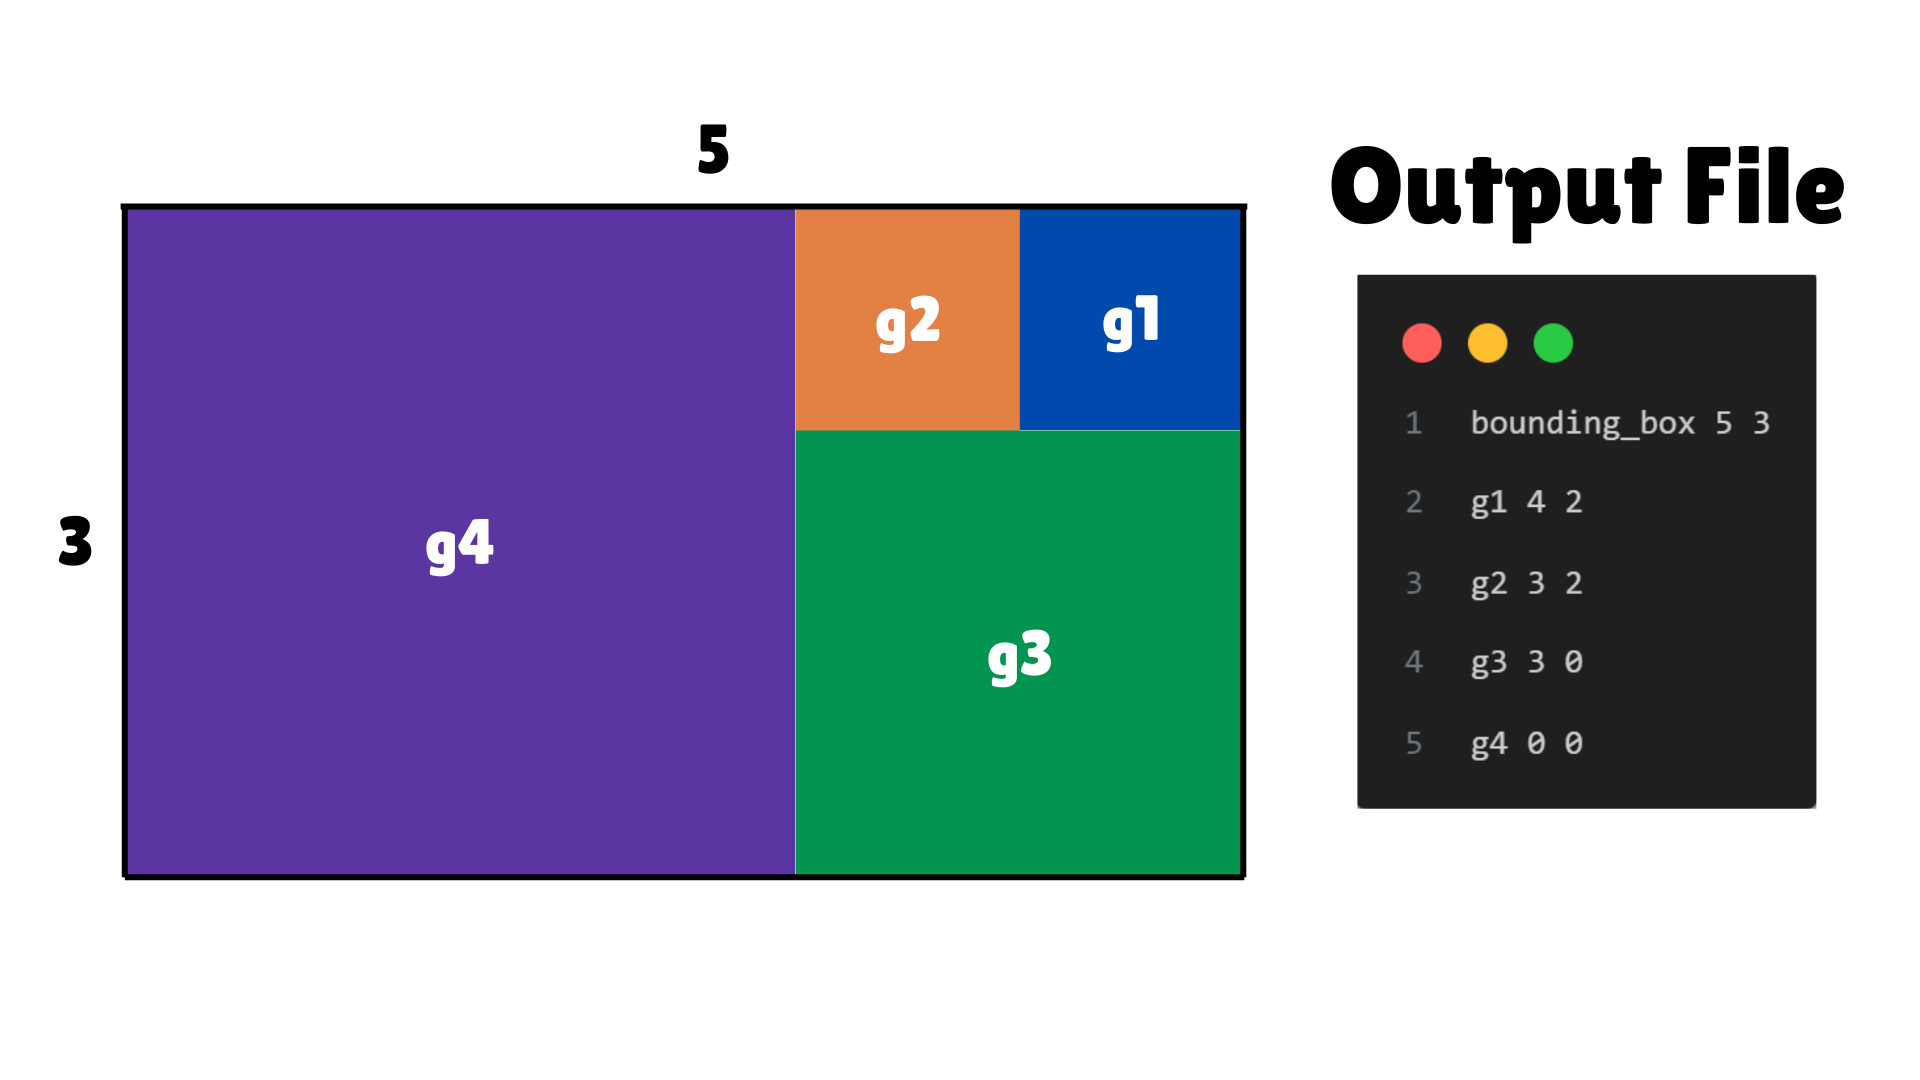
\includegraphics[width=0.8\linewidth]{BRoll/tc1_out_rep}
  % \captionof{figure}{Another figure}
  \label{fig:broll_mux}
\end{figure}

%%%%%%%%%%%%%%%%%%%%%%%%%%%%%%%%%%%%%%%%%%%%%%%%%%%%%%%%%%%%%%%
\newpage % Begin Page 2 %
%%%%%%%%%%%%%%%%%%%%%%%%%%%%%%%%%%%%%%%%%%%%%%%%%%%%%%%%%%%%%%%

\section{Modelling Gate Packing}
\subsection{What is Gate Packing ?}
\begin{flushleft}
In the context of gate level circuit designing, it refers to the process of arranging logic gates on a circuit board in order to minimize wasted space, reduce interconnection length and optimize the overall layout of the circuit board.
\end{flushleft}
\begin{flushleft}
Generalised gate packing is a very complex problem and involves multiple challenges such as placement and routing complexity, heat dissipation, design constraints due to fabrication processes, etc. but we will be tackling a simplified problem in this assignment.
\end{flushleft}
\subsection{Understanding the Problem Statement}
\begin{flushleft}
The problem statement models the gates as a set of n rectangles (provided as input for each test case) : \( \{g_{1},g_{2},...,g_{n}\}\) each represented by a pair of integers : \(g_{i} = (w_{i},h_{i})\) , where \(w_{i}\) and \(h_{i}\) are the width and the height of the \(i^{th}\) board. A given set of gates is said to be “correctly assigned" if no two gates have overlapping areas. The bounding rectangle is defined to be the smallest rectangle that encloses all gates and has the minimum area (out of all the possible “correctly assigned" cases).
\end{flushleft}

\begin{flushleft}
The program is supposed to output 2 things - The \(w\) and \(h\) of the bounding rectangle and the set of coordinates : \(\{ (x_{i},y_{i})\}^{i=n}_{i=1}\) - where \((x_{i},y_{i})\) denote the coordinate of the bottom left corner of the \(g_{i}\). A sample test case is given below :
(Note that every gate placed is in the original orientation provided by test case, i.e. re-orientation by rotation is disallowed)
\end{flushleft}

\begin{figure}[ht]
\centering
  \includegraphics[width=0.75\linewidth]{BRoll/tc2_rep}
  % \captionof{figure}{A figure}
   \label{fig:TC2}
   \captionof{figure}{Sample Test Case with 8 gates}
\end{figure}

%%%%%%%%%%%%%%%%%%%%%%%%%%%%%%%%%%%%%%%%%%%%%%%%%%%%%%%%%%%%%%%
% Begin Page 3 %
%%%%%%%%%%%%%%%%%%%%%%%%%%%%%%%%%%%%%%%%%%%%%%%%%%%%%%%%%%%%%%%

\begin{figure}[ht]
  \centering
  \includegraphics[width=0.75\linewidth]{BRoll/tc2_out_rep}
  % \captionof{figure}{Another figure}
  \label{fig:TC2_OUT}
  \captionof{figure}{Output of above sample case}
\end{figure}

\section{Algorithm Conceptualization and Design}
\begin{flushleft}
Our all three Algorithms solve the problem in a Y Direction Flipped manner.
Since the \((0,0)\) of our grid co-ordinates are taken in the top left (allowing us to iterate the grid in row-major order)
(which is different from the given problem statement where \((0,0)\) is taken in bottom right). Hence if any
correct packing is found by our algorithm then it will also work in the original problem statement.
\end{flushleft}
\begin{figure}[ht]
  \centering
  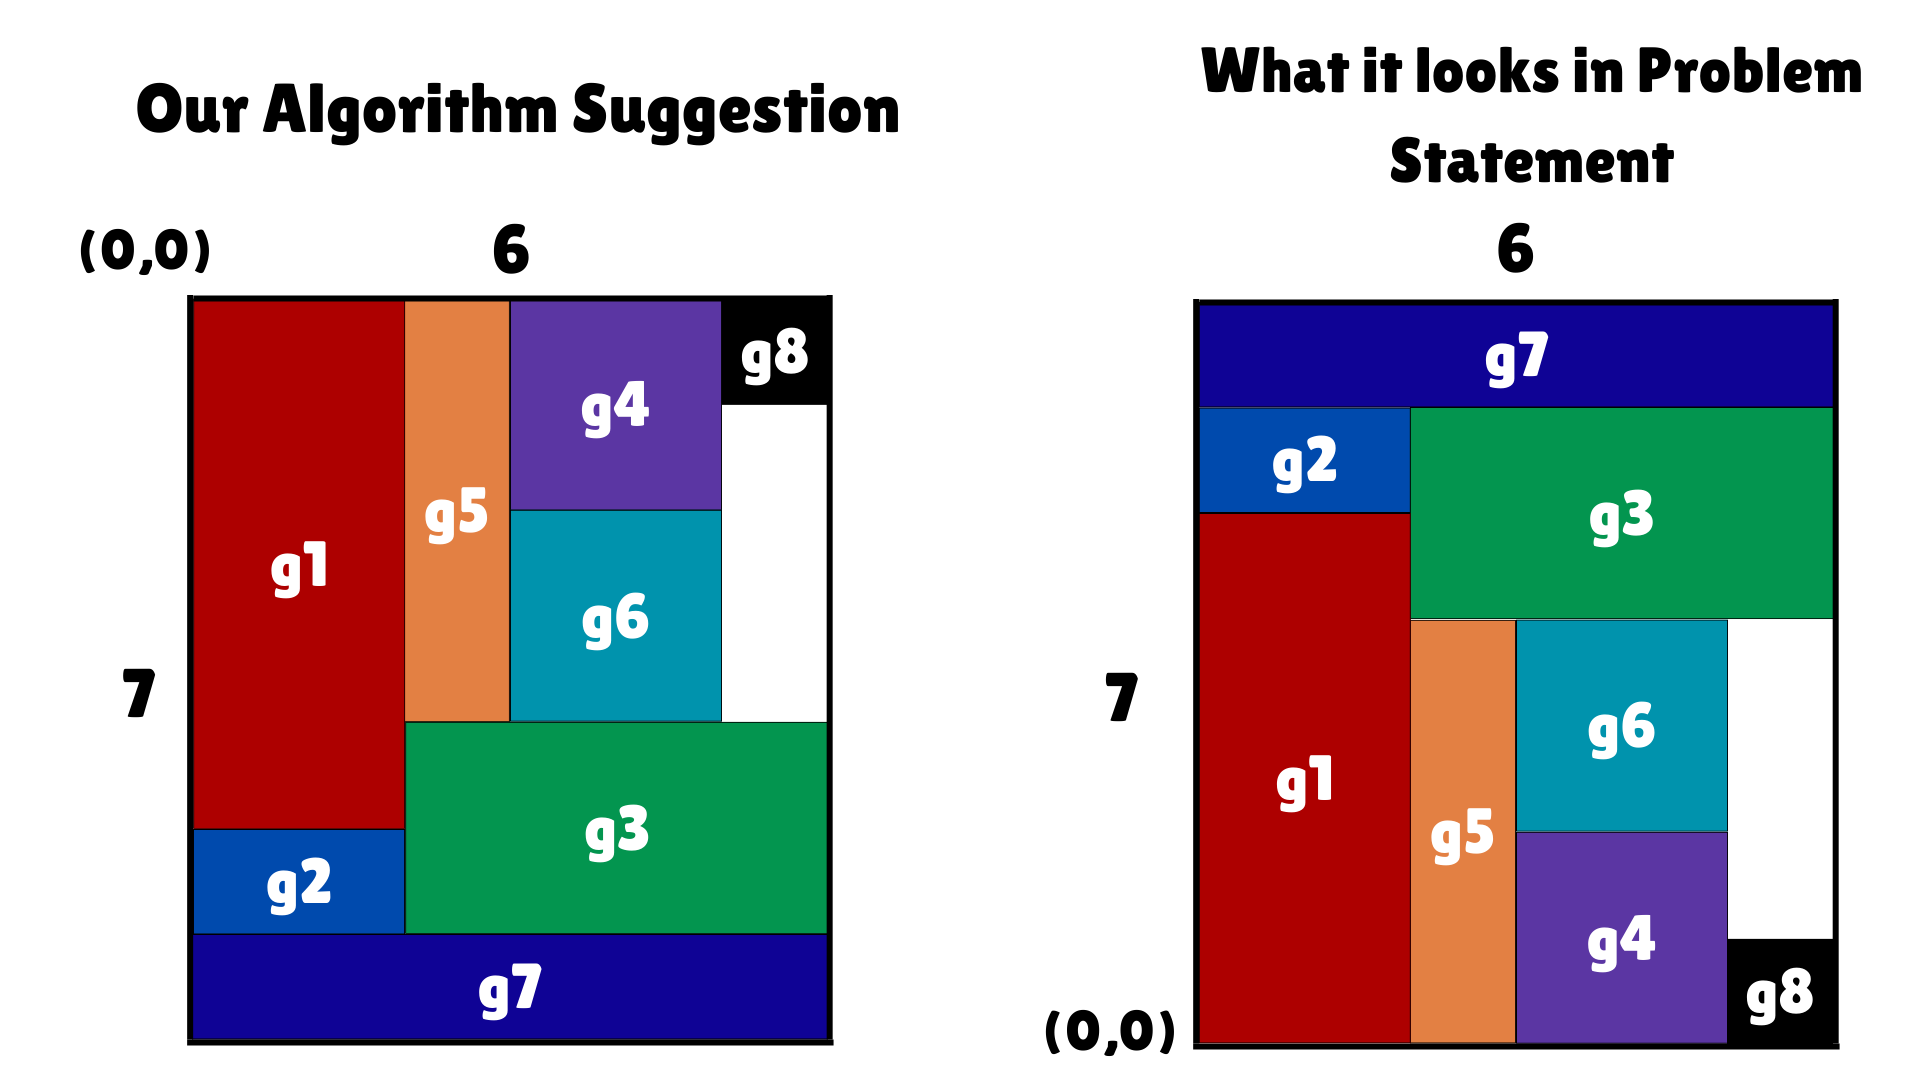
\includegraphics[width=0.8\linewidth]{BRoll/TC_Compare.png}
  % \captionof{figure}{Another figure}
  \label{fig:TC_Compare}
  \captionof{figure}{Y Flipped Output by our Algorithm}
\end{figure}

%%%%%%%%%%%%%%%%%%%%%%%%%%%%%%%%%%%%%%%%%%%%%%%%%%%%%%%%%%%%%%%
\newpage % Begin Page 4 %
%%%%%%%%%%%%%%%%%%%%%%%%%%%%%%%%%%%%%%%%%%%%%%%%%%%%%%%%%%%%%%%
\subsection{Naive Row Packing Algorithm}
\begin{flushleft}
This is a naive and one of the simplest ways to pack rectangles and involves following steps :
\begin{enumerate}
    \item Rectangles are sorted in decreasing order of height and width in respective priorities.
    \item Rectangles are added to a row from left to right until next rectangle does not fit.In such case the next rectangle is placed in the next row.
\end{enumerate}
\end{flushleft}

\subsection{Pixel Scan Algorithm}
\begin{flushleft}
The naive row packing algorithm can be enhanced by scanning the entire image (pixel by pixel) to identify a suitable location for every rectangle to be packed. Although this method introduces a slower process, further optimizations can be implemented in subsequent iteration. However, the packing logic remains quite rudimentary in its current state.
\begin{enumerate}
    \item Rectangles are sorted in decreasing order of height (and then by width).
    \item The algorithm implements a grid which stores value \((1/0)\) of every pixel.
    \item We then iterate through all the rectangles and, for each one, examine every pixel to determine whether the top-left and bottom-right corners of the rectangle are unoccupied. Additionally, we ensure that the rectangle does not extend beyond the boundaries defined by the grid.
    \item  We examine all the pixels within the potential rectangular region to ensure there is no overlap with any previously placed rectangles..
    \item Once we find a valid location we store location in the rectangle and mark those pixels as occupied \((1)\) in the grid.
    \end{enumerate}
\end{flushleft}

\subsection{Predictive-Pixel Scan Algorithm}
\begin{flushleft}
The Pixel Scan Algorithm can be optimized by reducing the number of iterations in the outermost loop. This can be achieved by leveraging the data from previously packed rectangles in the following manner :
\begin{enumerate}
    \item The improved algorithm involves sorting rectangles by height (and then by width) just like the previous algorithms.
    \item The algorithm implements a grid which stores 0 for unoccupied pixels and index value \(i\) of rectangle which occupies it.
    \item We iterate through the grid but instead of  looping through every pixel and checking its state , we check if a pixel is occupied or not. If it is occupied then we fetch the rectangle's width using the index and calculate the nearest right column which is not being covered by that rectangle and move our checking coordinates to that column (same row). If we exceed the width of image then we just move to the first column of the next row and continue with the iteration (This step makes the algorithm more efficient compared to before).
    \item If an empty pixel is identified, the corresponding sub-grid is evaluated to determine whether the given rectangle can be placed within it. If a covered pixel is encountered, a similar calculation to that in Step 3 is performed, after which we return to Step 3 to continue iterating through the grid..
    \item Once we find suitable position for the rectangle it fills the cells with index of the covering rectangle , sets the packed state of rectangle object, as well as its coordinates. 
\end{enumerate}

\end{flushleft}

% Flow Chart tikzpic %
\begin{center}
    

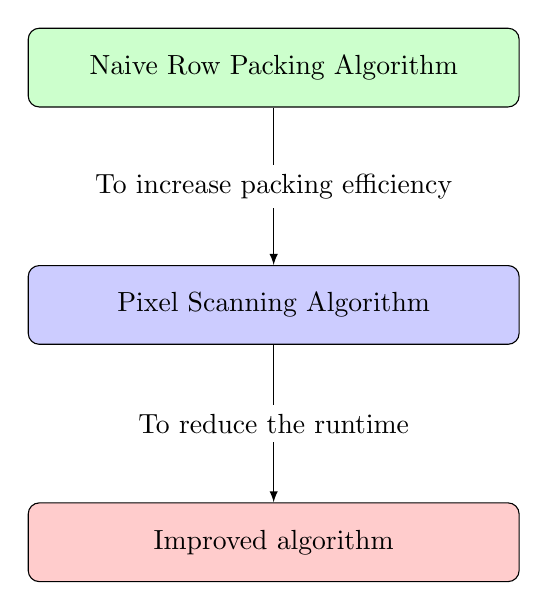
\begin{tikzpicture}[node distance= 2cm and 2cm][ht]

\node [startstop_wg] (s1) {Naive Row Packing Algorithm};
\node [startstop_wb,below = of s1] (s2) {Pixel Scanning Algorithm};
\node [startstop_wr, below = of s2] (s3) {Improved algorithm};

\path [line](s1) -- node[fill = white] {To increase packing efficiency}  (s2);
\path [line](s2) -- node[fill = white] {To reduce the runtime } (s3);

\end{tikzpicture}
\end{center}

\subsection{Proving Completion of algorithm}
\subsubsection{The Naive Row Packing algorithm}
\begin{flushleft}
    The correctness of this algorithm is trivial (from the way it is implemented) and can be shown by explicit construction in every case such as in Fig. 4.
\end{flushleft}
\subsubsection{Pixel Scan - Choice of Initial Bounding Box Dimensions}
\begin{enumerate}
    \item The first choice of number of rows and columns in the grid is done by calculating the total area of the rectangles to be packed.Initially, both the height and width are taken to be $\lfloor 1.1 \cdot \sqrt{A} \rfloor$ where A is the total area of gates to be packed :
    \begin{center}
         $W_{0}=H_{0}=\lfloor(1.1\cdot\sqrt{A} \rfloor$
    \end{center}
    Since there can be test cases where $W_{0}$ is less than the maximum width or $H_{0}$ is less than the maximum height , We set either dimension to be floor of \(1.5\) times the corresponding maximum gate dimension.
    \item In case no possible packing arrangement exists, we set the width to floor of 1.5 times the width of previous iteration until the packing is done :
    \begin{center}
        $W_{i+1}=\lfloor 1.5 \cdot W_{i} \rfloor$ 
    \end{center}
    \item Since we  have ensured that our rows are more than the maximum height of the gates, this process will terminate in a finite steps since a feasible upper bound on the number of columns is the sum of widths of all gates (as in the Naive Row Packing Algorithm).
\end{enumerate}

\begin{figure}[ht]
    \centering
    \begin{minipage}{.6\textwidth}
          \centering
          \includegraphics[width=1.0\linewidth]{Images/BRoll/annot.jpg}
          % \captionof{figure}{A figure}
          \label{fig:annot-1}
          \caption{Visualising Output of different algorithms}
          
               
    \end{minipage}
\end{figure}


\subsubsection{Optimizing the Algorithm - Introducing Multiple Iteration Logic}\label{subsubsec:MITL}

After a satisfactory packing arrangement is found we may try to find a better arrangement by varying the height and width of the grid if the time of single iteration is very small.
\begin{enumerate}
    \item We vary the width of the grid in intervals of 2.5\% of initial width and adjust height of grid accordingly (Upto a maximum of 20 times or A bound calculated by estimating runtime from the first single packing iteration, the minimum of two.)
    \item The algorithm runs another iteration on adjusted width and height. If the new output has a higher packing efficiency , then the maximum value and packing data is updated as a potential solution.
    \item The iterations stop once packing efficiency exceeds 95\% or runtime exceeds 2-3 seconds. The final packing with the highest packing efficiency is returned.
\end{enumerate}

\subsubsection{Correctness of Algorithm}
\begin{enumerate}
    \item In this variant, the small rectangles can have varying lengths and widths, and their orientation is fixed (they cannot be rotated). The goal is to pack them in an enclosing rectangle of minimum area, with no boundaries on the enclosing rectangle's width or height. The problem is NP-complete in general which means that the time required to solve the problem using any currently known algorithm increases rapidly and cannot be done in polynomial time.
    \item The methods of solving this problem can be categorized into two types: exact algorithms and heuristic algorithms. It is well-known that the exact algorithms can only solve small-scale instances within a reasonable computational time. 
    \item Therefore, we have proposed a new heuristic rectangle packing algorithm to maximize the area usage of the box while having decent runtime.The algorithm involves greedy placement of rectangles from large to small as well as efficient grid-checking to improve run time.
    \item If the largest rectangle remaining can't fit anywhere, we place it in a place that extends the pack region as little as possible.It is not perfect but it is easy to implement gives near perfect packing and decent runtime. 
\end{enumerate}
\newpage % Begin Page 4 %
\begin{figure}[ht]
    \centering
    \begin{minipage}{.5\textwidth}
          \centering
          \includegraphics[width=1.0\linewidth]{Images/BRoll/complexity_classes.png}
          % \captionof{figure}{A figure}
          \label{fig:4bit-res1_sb}
          \caption{P vs NP Problems }
      
          
      \end{minipage}
\end{figure}

\section{Project Structure \& Design Decisions}
\subsection{Files of Code Directory}
\begin{flushleft}
    In addressing the problem statement, which encompassed the Input/Output requirements, Test Case generation, and analysis, we adopted a structured approach. Multiple Python files were meticulously made to manage different aspects of the problem. Each file was documented and organized to handle specific components of the solution, ensuring clarity and readability in the overall implementation even for a third party. Detail of particular files are given below :
\end{flushleft}
\begin{enumerate}
    \item \textbf{code\_timer.py} : This module defines the wrapper functions time\_it and time\_it\_no\_out, which are utilized for measuring the execution time of functions. These functions assist in graphical analysis by providing precise timing information.
    \item \textbf{IO\_Parser.py} : This module facilitates the parsing of input and output, converting data related to packed rectangles into a user-readable format and vice versa.
    \item \textbf{Pack\_by\_Pixels.py} : This module contains the implementation of the Naive Row Packing, Pixel Scanning, and Predictive Pixel Scanning algorithms.
    \item \textbf{project\_constants.py} : As the number of constants used across the programs increased, a dedicated Python file was created to manage and track these constants. This organization facilitated the simultaneous testing of multiple test cases by generating the corresponding file paths. Additionally, it enabled adjustments to the implementation to optimize performance and achieve better results.
    \item \textbf{Rect.py} : This module defines a custom class -\(Rect\), which represents the gates utilized in the packing algorithms. It also includes the Rec\_Data\_Analysis method, which generates key statistics about the rectangles within a given test case.
    \item \textbf{test\_code.py} : This file defines the logic for both single and multiple iterations and includes various methods for analyzing different types of test cases and generating corresponding output files. It serves as the central component of the assignment, orchestrating the overall operation and ensuring cohesive functionality throughout the process.
    \item \textbf{testcase\_gen.py} : This component assists in generating both single and multiple test cases, tailored according to gate frequency. It incorporates three distinct modes for test case generation, utilizing the NumPy library for efficient data handling. Additionally, it provides functionality to delete Input/Output files associated with previous test cases, ensuring a clean and organized testing environment. 
    \item \textbf{text\_analysis.py} : This file use Matplotlib to analyze the report files generated in the preceding files. This analysis involved visualizing the data through various graphs, facilitating a comprehensive understanding of the performance metrics and outcomes.
\end{enumerate}

\subsection{Multiple vs Single Iteration - Which is better ?}\label{subsec:MSP}
\begin{flushleft}
    After implementing the Predictive Pixel Scan algorithm, we encountered a dilemma 
    whether to run multiple iterations for cases where run time is smaller in order to go for higher packing efficiency or let the implementation be naturally fast for all frequency of gates.
\end{flushleft}
\begin{flushleft}
    It is important to note that the behaviour of multi iteration logic becomes the same as that of single iteration above a certain threshold of frequency of gates.
    This is due to the implementation explained in 2.4.3 - Since the packing efficiency as well as time (for a single successful packing) grows with the number of gates , the code exits due to point 3 at the first iteration itself.
\end{flushleft}
\begin{flushleft}
    After crunching some data across multiple test cases we came to the conclusion that when the gate frequency is less than 200-250, the gain in packing efficiency is really noticeable only for \(<50\) gates.Thus the trade-off \(~20\) times more runtime is only viable if any theoretical/practical (industrially) cost function (used for analysing output) weighs heavily towards packing efficiency. 
\end{flushleft}
\begin{flushleft}
    Thus if we prioritise towards Run Time, say we want to generate multiple designs very quickly then single iteration is useful. However if say a company wants to create one design which will be produced on a massive scale, the delta gain in packing efficiency will improve the cost of manufacturing by a lot, in which case we may even run more than multi iteration is a better solution. Since for our assignment purposes the final runtime isn't as significant as long it is fast, we use multi iteration logic for analysing our test cases. 
\end{flushleft}

%%%%%%%%%%%%%%%%%%%%%%%%%%%%%%%%%%%%%%%%%%%%%%%%%%%%%%%%%%%%%%%
\newpage % Begin Page 5 %
%%%%%%%%%%%%%%%%%%%%%%%%%%%%%%%%%%%%%%%%%%%%%%%%%%%%%%%%%%%%%%%

\section{Time Complexity \& Packing Efficiency Analysis}
\subsection{Naive Row Packing Algorithm}
\begin{flushleft}
    The time complexity of this naive algorithm standalone is \(O(n)\) (where n is the number of gates) since it only involves finding the maximum height of a rectangle and packing them side-by-side in a single iteration over all rectangles, according to the widths (as visible in the code below)
\end{flushleft}
\begin{flushleft}
    However our IO-Parser also sorts the rec\_data (as mentioned before) while preparing it to pass to a packing algorithm. Hence the overall implementation has a time complexity of \(O(n\log{n})\).  sorting doesn't provide any algorithmic benefit, the sorting can be suppressed by an argument if this algorithm has to be used.
\end{flushleft}
\begin{lstlisting}[language=Python, caption = Naive Row Algorithm's Python Implementation]
def Pack_by_Pixel_v0(rec_data,h_max):
    x,y = 0,0
    cells_packed, max_rows_used, max_cols_used = 0, h_max, 0
    rdata = deepcopy(rec_data)
    
    for i in range(len(rdata)):
        rdata[i].set_pos(x,y)
        rdata[i].packed()
        x += rdata[i].width
        cells_packed += (rdata[i].width)*(rdata[i].height)
    
    max_cols_used = x
    
    return rdata,[cells_packed,max_rows_used,max_cols_used],True
\end{lstlisting}

\subsection{Pixel Scan Algorithm}
\begin{flushleft}
    The time complexity of this heuristic algorithm is not easy to calculate systematically since the grid will change dynamically with rectangle placements. However we can claim a loose upper bound to be \(O(n^{2})\) by the following logic :
\end{flushleft}

\begin{enumerate}
    \item Suppose the outer loops (Line 9 and 13) run over the entire grid for every rectangle object (loop on Line 7). Hence it has to run over \(A_{0}\) pixels (an upper bound) , where \(A_{0} = W_{0}\cdot H_{0}\) , is the area of initial bounding box guess.
    \item Suppose for every possible empty pixel it has to scan \(A_{r}\) pixels , \(A_{r}\) being the area of the rectangle being packed.If it finds that all \(A_{r}\) pixels are empty then runs on them again,marking them as occupied. Hence running over \(2\cdot A_{r}\) pixels for each rectangle.
    \item Therefore, a worst case upper bound of pixels which we need to iterate is given by : 
    \[ \sum_{r = 1}^{n}O(2\cdot A_{o}\cdot A_{r}) \leq O( A_{o}\cdot n\cdot A_{max})\approx O(A_{Tot}\cdot n\cdot 10^{4}) \approx O\left(n\cdot\frac{10^{4}}{4} \cdot n\right) = O(n^{2}) 
    \] Here \(A_{o}\) is taken approximately to be \(A_{Tot}\) (The total area of gates that have to be placed), which is further approximated as \(\frac{A_{max}}{4}\) (Since our dimensions are drawn independently from a normal distribution with mean at half of maximum dimension). \(A_{max} = 10^{4}\) by the constraints of problem statement. 
\end{enumerate}

\begin{lstlisting}[language=Python, caption= Outer loops of Pixel Scan Implementation]
def Pack_by_Pixel_v1(rec_data,Im_Width,Im_Height):
    
    rdata = deepcopy(rec_data)
    cells_packed, max_rows_used, max_cols_used = 0, 0, 0
    Im_Data = [[0]*Im_Width for r in range(Im_Height)]
    
    for i in range(len(rdata)):
        rec_done = False
        for y in range(Im_Height):
            if(y+rdata[i].height > Im_Height or rec_done):
                break
            else:
                for x in range(Im_Width):
                    if(x+rdata[i].width > Im_Width):
                        break
                    # [Internal Loops ...]
        if(not rec_done):
            return -1,None,None                    
    
    return rdata,[cells_packed,max_rows_used,max_cols_used],True
\end{lstlisting}
\begin{lstlisting}[language=Python, caption= Internal Loops of Pixel Scan Implementation]
# [Internal Loops ...]
if(Im_Data[y][x] == 0 and Im_Data[y+rdata[i].height-1][x+rdata[i].width-1] == 0):
    isvalid = True
    for r in range(y,y+rdata[i].height):
        if(isvalid):
            for c in range(x,x+rdata[i].width):
                if(Im_Data[r][c] == 1):
                    isvalid = False
                    break
        else:
            break
    if(isvalid):
        # [Successful Packing Loops]
        # [Marks the grid location as occupied]
        # [Updates the attributes of Rec Object]
        rec_done = True
        break
\end{lstlisting}

\newpage
\subsection{Predictive Pixel Scan}
\begin{flushleft}
    The time complexity of this heuristic algorithm is even harder to calculate systematically since now the pixel finding loop (Line 10) has iterations dependent on the widths of already packed gates. However the upper bound can still proven to be \(O(n^{2})\) by the following logic :
    \begin{enumerate}
    \item For the worst case scenario, the only difference between this and the previous algorithm is that for a given row, instead of scanning it entirely it only scans at gaps of the already filled rectangle's widths.
    \item Hence instead of Scanning \(W_{0}\) pixels per row , It will on average scan \(\approx \frac{W_{0}}{\varphi}\) pixels per row, \(\varphi\) being the average width of gates placed in a row.
    \item \(\varphi\) can be approximated since we draw our samples from a normal distribution with mean at half of maximum dimension. Hence we can take \(\varphi \approx 50\).
    \item This has an interesting implication, since instead of going over \(A_{0}\) pixels for each rectangle, we only run over \(\frac{A_{0}}{\varphi}\) pixels. Since \(\varphi\) doesn't depend on order of n, hence we can further use the logic of Pixel Scan to calculate time complexity as \(O(n^{2})\) (Ignoring \(\varphi\) as a constant during the big-\(O\) calculation.)
    \item Despite having same \(O(n^{2})\) time complexity , this performs much better than previous algorithm which is explained later.
\end{enumerate}
\end{flushleft}
\begin{lstlisting}[language=Python, caption= Outer loops of Predictive Pixel Scan Implementation]
def Pack_by_Pixel_v2(rec_data,Im_Width,Im_Height):
    rdata = deepcopy(rec_data)
    cells_packed,max_rows_used,max_cols_used = 0,0,0
    Im_Data = [[0]*Im_Width for r in range(Im_Height)]
    Im_Rec_Data = {rdata[i].index : rdata[i] for i in range(len(rdata))}
        
    for i in range(len(rdata)):
        rec_done = False
        x,y = 0,0
        for _inf_it in count(0,1):
            if (y + rdata[i].height > Im_Height or rec_done):
                break
            else:
                if(x + rdata[i].width > Im_Width):
                    x,y = 0,y+1
                    continue
                else:
                    # [Internal Loops ...]

        if(not rec_done):
            return -1,None,None                    

    return rdata,[cells_packed,max_rows_used,max_cols_used],True

\end{lstlisting}
\begin{lstlisting}[language=Python, caption= Inner loops of Predictive Pixel Scan Implementation]
# [Internal Loops ...]
if(Im_Data[y][x] == 0):
    if(Im_Data[y+rdata[i].height-1][x+rdata[i].width-1] == 0):
        isvalid = True
        for r in range(y,y+rdata[i].height):
            if(isvalid):
                for c in range(x,x+rdata[i].width):
                    if(Im_Data[r][c] != 0):
                        isvalid = False
                        row_notvalid,col_notvalid = r,c
                        break                                            
            else:
                break        
        if(isvalid):
            # [Successful Packing Loops]
            # [Marks the grid location as occupied]
            # [Updates the attributes of Rec Object]
            rec_done = True
            break
        else:
            w_enc = # Width of Rectangle stored at invalid position
            x_enc = # X of Rectangle stored at invalid position
            x = x_enc + w_enc 
            continue        
    else:
        x = x + rdata[i].width
        continue
else:
    w_enc = # Width of Rectangle stored at (x,y) [Line 2]
    x_enc = # X of Rectangle stored at (x,y) [Line 2]
    x = x_enc + w_enc 
    continue
\end{lstlisting}
\begin{flushleft}
    Here we must mention that the order of \(n\) in our problems is at max 1000, which isn't large enough for good asymptotic analysis. Thereby the constants of implementation matter and \(\varphi\) is the reason that our second algorithm is \textbf{practically much faster} than the previous implementation. 
\end{flushleft}
\begin{flushleft}
    Additionally \(\varphi\) need not be a constant but the only important aspect (for theoretical calculations) is that it is independent of \(n\). Practically we can see the improvement by plotting Run Time as we increase the number of gates \((n)\) as shown below. (It is important to note that runtime of cases less than 200 seems to be higher than cases above 200 in the graph. This implementation decision is explained later)
\end{flushleft}
\begin{figure}[ht]
    \centering
    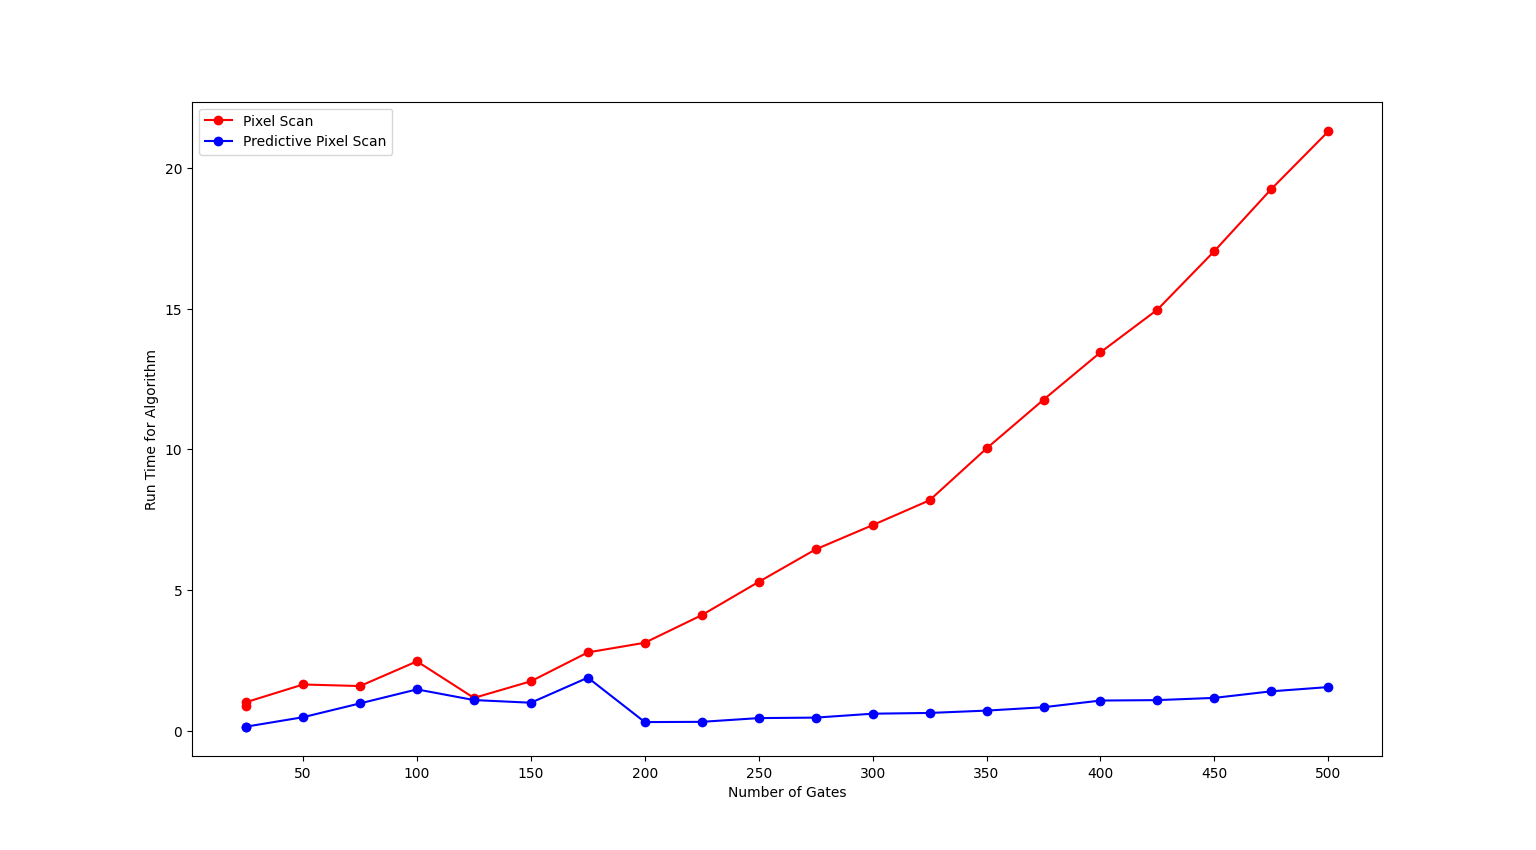
\includegraphics[width=1.0\linewidth]{Images/BRoll/V1V2_Comp.png}
    \caption{Run Time Comparison of 2 Implementations}
    \label{fig:enter-label}
\end{figure}

\newpage
\subsection{Plot of \(t\) vs \(n\) \& \(\eta\) vs \(n\) for Test Cases}
\begin{flushleft}
    The following table shows the runtime and packing efficiency for the test cases given on Piazza. Our algorithm performs sufficiently fast and gives good packing efficiency for these test cases.
\end{flushleft}
\begin{center}
\begin{table}[ht]
\centering
\begin{tabular}{|
>{\columncolor[HTML]{FFFC9E}}c |
>{\columncolor[HTML]{FFFC9E}}c |
>{\columncolor[HTML]{FFFC9E}}c |
>{\columncolor[HTML]{FFFC9E}}c |}
\hline
\cellcolor[HTML]{DAE8FC}Test Case & \cellcolor[HTML]{DAE8FC}\begin{tabular}[c]{@{}c@{}}Number of Gates \((n)\)\end{tabular} & \cellcolor[HTML]{DAE8FC}\begin{tabular}[c]{@{}c@{}}Runtime in Seconds \((t)\)\end{tabular} & \cellcolor[HTML]{DAE8FC}\begin{tabular}[c]{@{}c@{}}Packing Efficiency \((\eta)\)\end{tabular} \\ \hline
{\color[HTML]{000000} 1}     & {\color[HTML]{000000} 3}                                                              & 0.005484                                                                                 & 0.818181                                                                                    \\ \hline
{\color[HTML]{000000} 2}     & {\color[HTML]{000000} 3}                                                              & 0.009657                                                                                 & 0.933333                                                                                    \\ \hline
{\color[HTML]{000000} 3}     & {\color[HTML]{000000} 10}                                                             & 0.008263                                                                                 & 0.902778                                                                                    \\ \hline
{\color[HTML]{000000} 4}     & \cellcolor[HTML]{FFFC9E}{\color[HTML]{000000} 5}                                      & 0.004607                                                                                 & 0.845238                                                                                    \\ \hline
\cellcolor[HTML]{FFFC9E}5    & \cellcolor[HTML]{FFFC9E}35                                                            & 0.004479                                                                                 & 0.952381                                                                                    \\ \hline
\end{tabular}
\caption{\(t\) and \(\eta\) on Sample cases (provided on Piazza)}
\label{table:1}
\end{table}
\end{center}
\begin{flushleft}
    To stress test our code, we automated creation of Test Cases using two-three methods. Firstly we ran our algorithm on test cases where the gate frequency
    ranges from 5 to 1000 (at a difference of 5 gates) to check how the packing efficiency as well as run time varies with increasing the number of gates \((n)\) :
\end{flushleft}

\newpage
\begin{figure}[ht]
    \centering
    \begin{minipage}{1.0\linewidth}
        \centering
        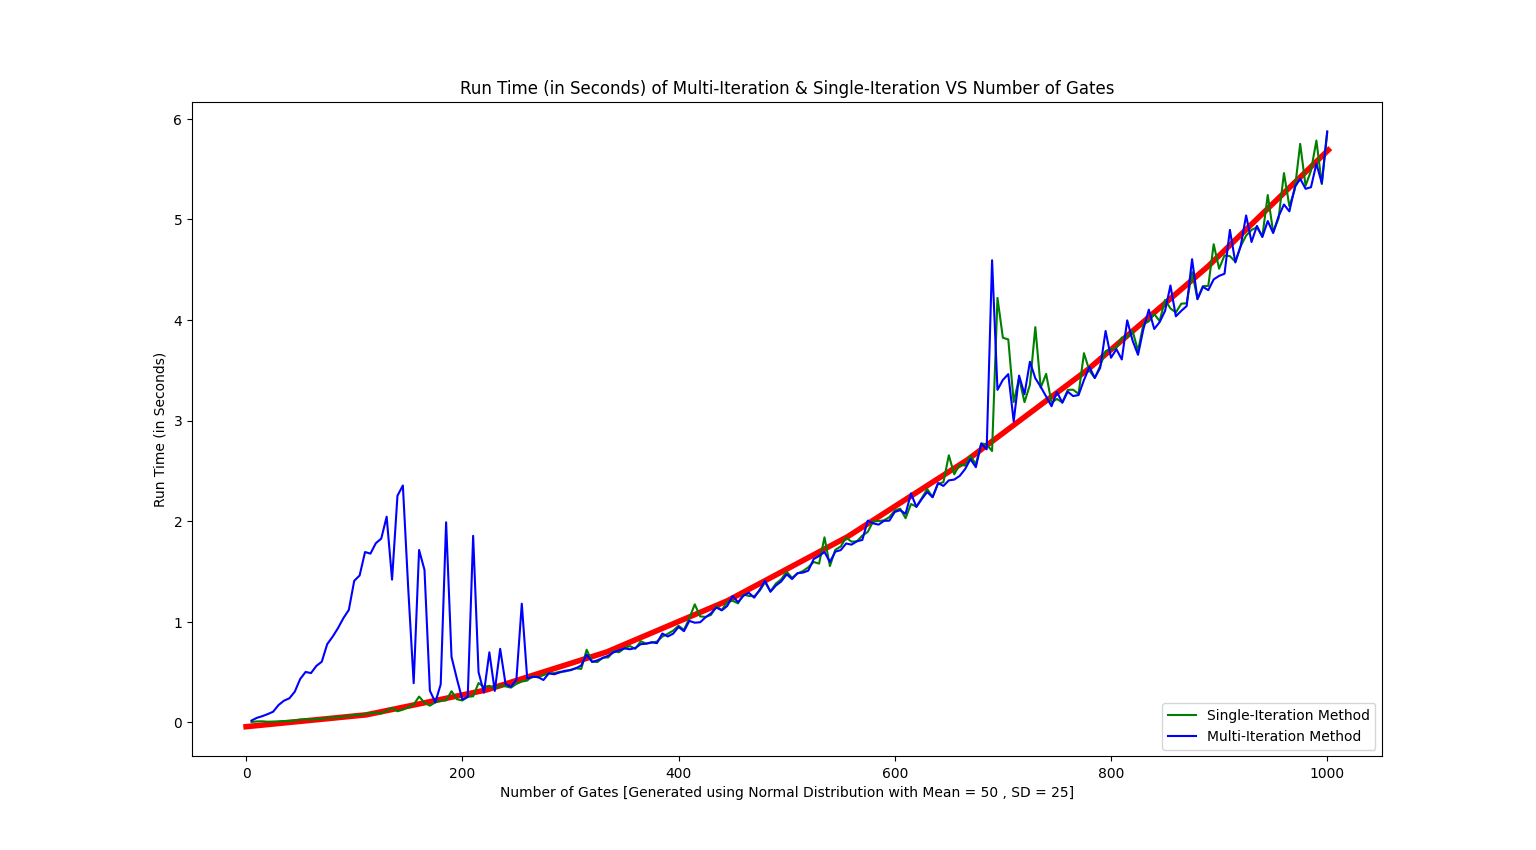
\includegraphics[width=0.9\linewidth]{Images/BRoll/MP_SP_Comparison_Run_Time.png}
        % \captionof{figure}{A figure}
        \label{fig:mp-sp-runtime}
        \caption{Run Time vs Number of Gates}    
    \end{minipage}
    \begin{minipage}{1.0\linewidth}
        \centering
        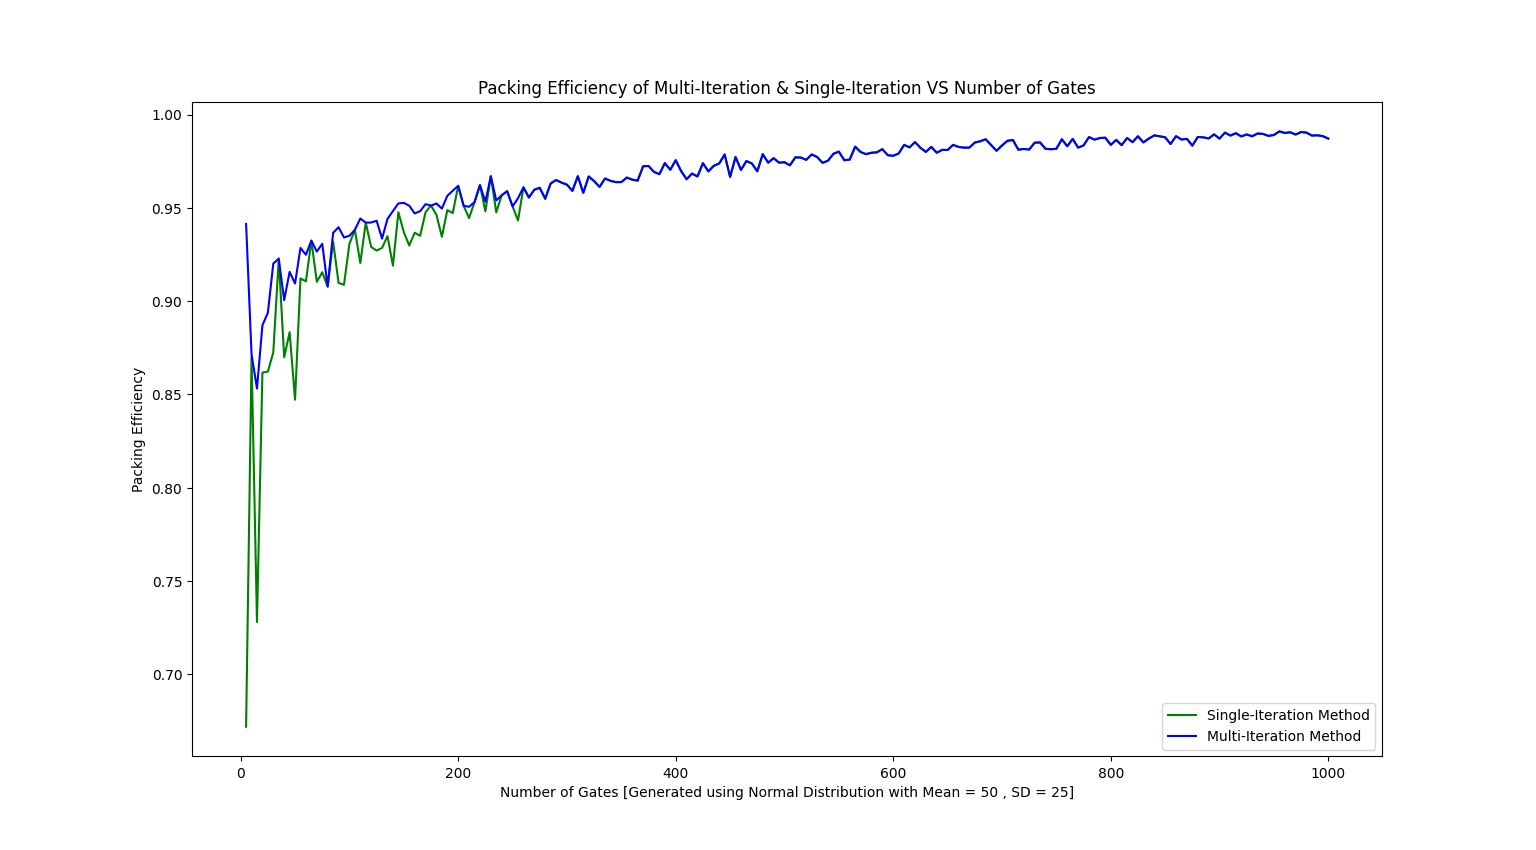
\includegraphics[width=0.9\linewidth]{Images/BRoll/MP_SP_Comparison_Pack_Eff.png}
        % \captionof{figure}{A figure}
        \label{fig:mp-sp-peff}
        \caption{Packing Efficiency vs Number of Gates}    
    \end{minipage}
\end{figure}
\begin{flushleft}
    The multi iteration method only runs 20 or so more iterations of the same algorithm (in nearby widths) in hope of finding better packing.The observations from the above graphs are:\\
    \subsubsection{Runtime :}
    \begin{enumerate}
        \item The runtime for both single and multi iteration is approximately quadratic in nature with respect to number of gates. This is as expected and the best fit quadratic curve has following expression (using NumPy polyfit):
        \[T(n) = 5.248\cdot 10^{-6}\cdot n^{2} + 4.773\cdot 10^{-4}\cdot n -0.04536\]
        Where \(T(n)\) is the runtime on \(n\) gates Test Case (in seconds)
        \item There is deviation in multi and single iteration for less than 300 gates which is as expected as per the discussion in \hyperref[subsec:MSP]{Section \ref*{subsec:MSP}}. For higher gate frequency they both tend to show same behaviour.
        \item A peak is observed near \(n\) = 700 - 750 but in magnitude terms, the deviation from expected behaviour is only of 1-2 s. This can be accounted for randomness of the test case generation and the fact that for the given plot , we only generated single case for each gate frequency.
    \end{enumerate}
    \subsubsection{Packing Efficiency:}
    \begin{enumerate}
        \item The packing efficiency is almost same($>$ 0.95) for multi and single iteration for more than 300 gates due to the explanation of \hyperref[subsec:MSP]{Section \ref*{subsec:MSP}}.
        \item For less than 300 gates the packing efficiency of multiple iteration is greater than single iteration. This is because of the logic of multiple iteration implementation discussed in \hyperref[subsubsec:MITL]{Subsection \ref*{subsubsec:MITL}}.
    \end{enumerate}


\end{flushleft}

\subsection{Average Runtime and Packing Efficiency for Multiple Testcases}

\begin{table}[ht]

\centering
\begin{tabular}{|
>{\columncolor[HTML]{FFFC9E}}c |
>{\columncolor[HTML]{FFFC9E}}c |
>{\columncolor[HTML]{FFFC9E}}c |
>{\columncolor[HTML]{FFFC9E}}c |}
\hline
\cellcolor[HTML]{DAE8FC}SNo. & \cellcolor[HTML]{DAE8FC}\begin{tabular}[c]{@{}c@{}}Number of Gates $(n)$\end{tabular} & \cellcolor[HTML]{DAE8FC}\begin{tabular}[c]{@{}c@{}}Average Runtime in Seconds $(t)$\end{tabular} & \cellcolor[HTML]{DAE8FC}\begin{tabular}[c]{@{}c@{}}Packing Efficiency $(\eta)$\end{tabular} \\ \hline
{\color[HTML]{000000} $1$}     & {\color[HTML]{000000} $25$}                                                             & $0.109190$                                                                                         & $0.898202$                                                                                    \\ \hline
{\color[HTML]{000000} $2$}     & {\color[HTML]{000000} $100$}                                                            & $1.802440$                                                                                         & $0.939640$                                                                                    \\ \hline
{\color[HTML]{000000} $3$}     & {\color[HTML]{000000} $250$}                                                            & $0.560971$                                                                                         & $0.956785$                                                                                    \\ \hline
{\color[HTML]{000000} $4$}     & \cellcolor[HTML]{FFFC9E}{\color[HTML]{000000} $1000$}                                   & $7.327116$                                                                                         & $0.989691$                                                                                    \\ \hline

\end{tabular}
\caption{Average $t$ \& $\eta$ for $100$ cases for different $n$ : $\mu = 50$, $\sigma = 25$}
\label{table:2}
\end{table}
\begin{table}[ht]
\begin{tabular}{|
>{\columncolor[HTML]{FFFC9E}}c |
>{\columncolor[HTML]{FFFC9E}}c |
>{\columncolor[HTML]{FFFC9E}}c |
>{\columncolor[HTML]{FFFC9E}}c |}
\hline
\cellcolor[HTML]{DAE8FC}SNo. & \cellcolor[HTML]{DAE8FC}\begin{tabular}[c]{@{}c@{}}Number of Gates $(n)$\end{tabular} & \cellcolor[HTML]{DAE8FC}\begin{tabular}[c]{@{}c@{}}Average Runtime in Seconds $(t)$\end{tabular} & \cellcolor[HTML]{DAE8FC}\begin{tabular}[c]{@{}c@{}}Packing Efficiency $(\eta)$\end{tabular} \\ \hline
{\color[HTML]{000000} $1$}     & {\color[HTML]{000000} $25$}                                                             & $0.111734$                                                                                         & $0.880246$                                                                                    \\ \hline
{\color[HTML]{000000} $2$}     & {\color[HTML]{000000} $100$}                                                            & $1.321254$                                                                                         & $0.927841$                                                                                    \\ \hline
{\color[HTML]{000000} $3$}     & {\color[HTML]{000000} $250$}                                                            & $0.984085$                                                                                         & $0.956785$                                                                                    \\ \hline
{\color[HTML]{000000} $4$}     & \cellcolor[HTML]{FFFC9E}{\color[HTML]{000000} $1000$}                                   & $4.771615$                                                                                         & $0.977463$                                                                                    \\ \hline
\end{tabular}
\caption{Average $t$ \& $\eta$ for $100$ cases for different $n$ : $\mu = 50$, $\sigma = 10$}
\label{table:3}
\end{table}
\begin{flushleft}
The above test cases, gate dimensions have been generated using normal distribution.
Since our algorithm revisits grid and packs shorter and less leaner rectangles in available spaces, when the $\sigma$ is low, then such rectangles generate with less probability hence the worse packing efficiency. 
\end{flushleft}
%%%%%%%%%%%%%%%%%%%%%%%%%%%%%%%%%%%%%%%%%%%%%%%%%%%%%%%%%%%%%%%%%
% fafasf
%%%%%%%%%%%%%%%%%%%%%%%%%%%%%%%%%%%%%%%%%%%%%%%%%%%%%%%%%%%%%%%%%
\newpage
\section{Visualising Output on Multiple Test Cases}

\subsection{Test Case 1}
\begin{center}
\begin{tabular}{|c|c|c|}
    \hline
    \rowcolor[HTML]{DAE8FC} Gate No. &
    Input \((w,h)\)                                    & Output \((x,y)\)   \\ \hline
    \rowcolor[HTML]{FFFC9E} {\color[HTML]{000000} \(1\)} &
    {\color[HTML]{000000} \((3,10)\)}                         & {\color[HTML]{000000} \((0,0\))}    \\ \hline
    \rowcolor[HTML]{FFFC9E} 
    {\color[HTML]{000000} \(2\)} &
    {\color[HTML]{000000} \((8,3)\)}                         & {\color[HTML]{000000} \((3,0)\)}      \\ \hline
     \rowcolor[HTML]{FFFC9E} 
     {\color[HTML]{000000} \(3\)} &
    {\color[HTML]{000000} \((6,6)\)}                         & {\color[HTML]{000000} \((3,6\))}      \\ \hline
    
\end{tabular}
\end{center}
\begin{center}
\textbf{Bounding Box Dimension : Width = \(11\) , Height = \(10\)}    
\end{center}
\begin{figure}[ht]
    \centering
    \begin{minipage}{.6\textwidth}
          \centering
          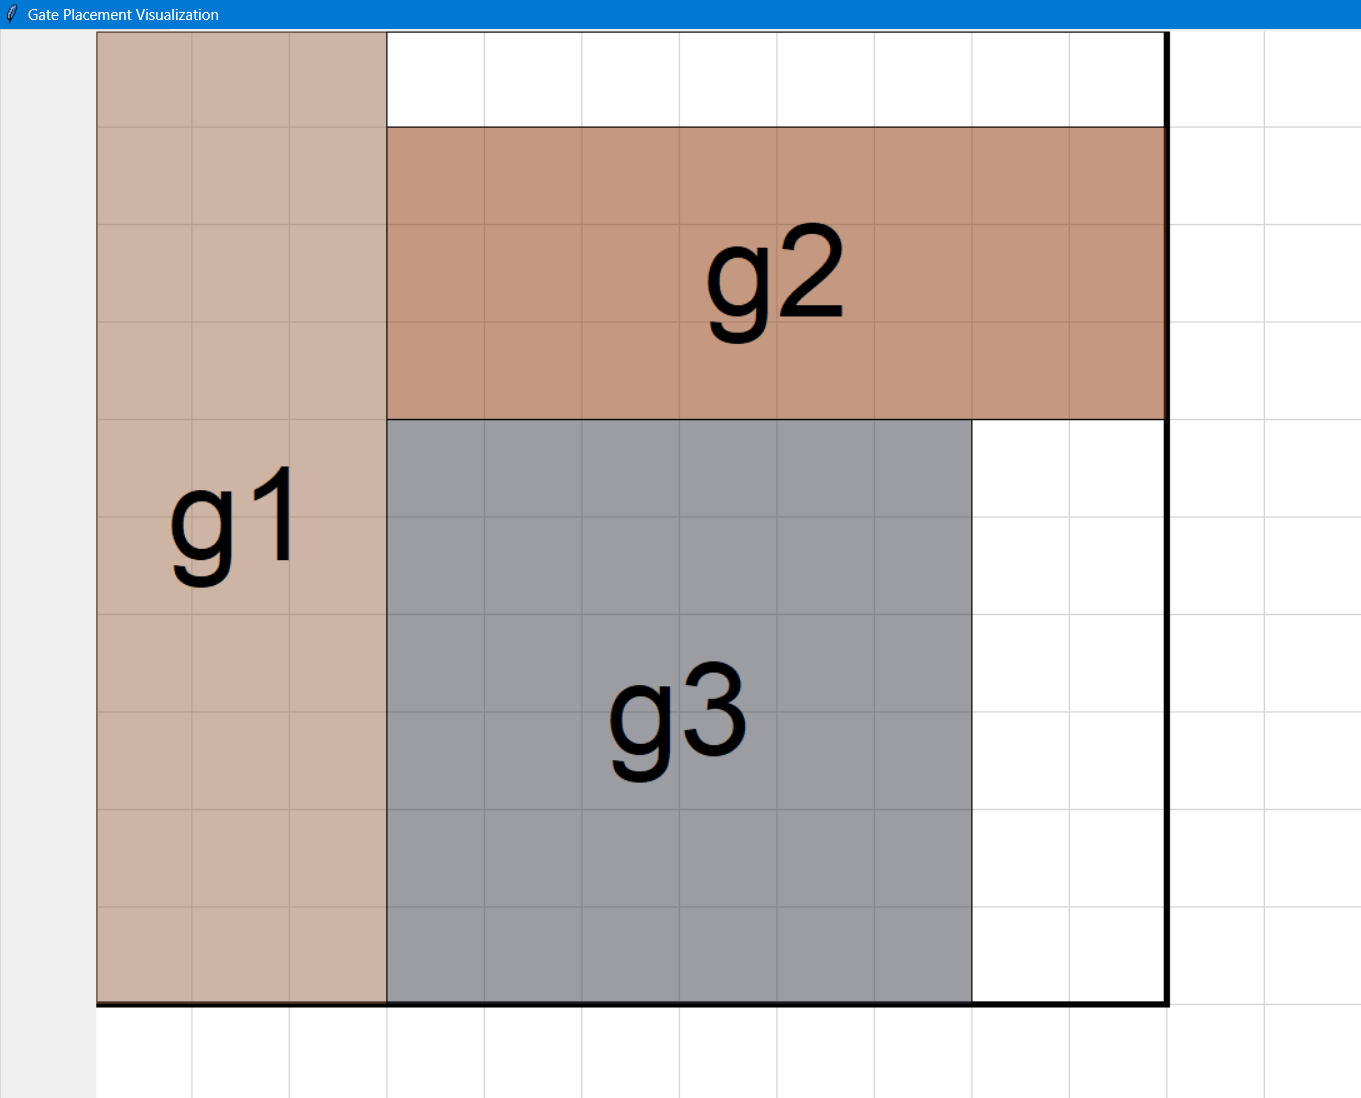
\includegraphics[width=1.0\linewidth]{Images/BRoll/Our_Packing_TC1.png}
          % \captionof{figure}{A figure}
          \label{fig:tc-1}
          \caption{Gate Packing }
      
          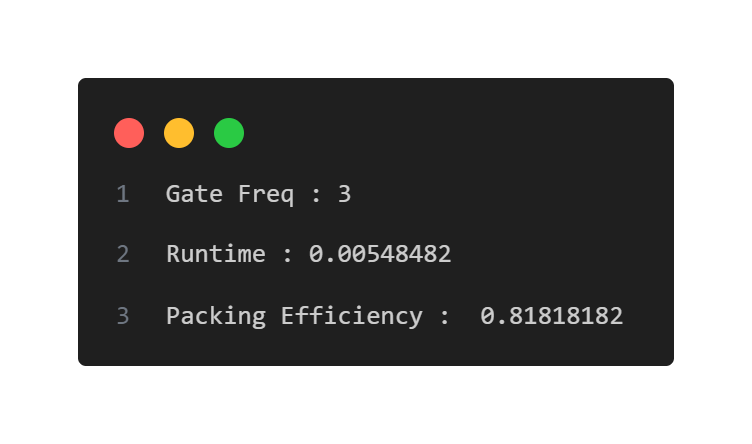
\includegraphics[width=0.95\linewidth]{Images/BRoll/Our_Packing_TC1_Report.png}
          % \captionof{figure}{A figure}
          \label{fig:tcr-1}
          \caption{Report}
          \centering 
      \end{minipage}
    \end{figure}
    
\newpage
\subsection{Test Case 2}
\begin{center}
\begin{tabular}{|c|c|c|}
    \hline
    \rowcolor[HTML]{DAE8FC} Gate No. &
    Input \((w,h)\)                                    & Output \((x,y)\)   \\ \hline
    \rowcolor[HTML]{FFFC9E} {\color[HTML]{000000}\(1\)} &
    {\color[HTML]{000000}\((3,4)\)}                         & {\color[HTML]{000000}\((0,0)\)}    \\ \hline
    \rowcolor[HTML]{FFFC9E} 
    {\color[HTML]{000000} \(2\)} &
    {\color[HTML]{000000}\((5,2)\)}                         & {\color[HTML]{000000}\((3,0)\)}      \\ \hline
     \rowcolor[HTML]{FFFC9E} 
     {\color[HTML]{000000} \(3\)} &
    {\color[HTML]{000000}\((2,3)\)}                         & {\color[HTML]{000000}\((0,4)\)}      \\ \hline
    
\end{tabular}
\end{center}
\begin{center}
\textbf{Bounding Box Dimension : Width = \(5\) , Height = \(6\)}   
\end{center}
\begin{figure}[ht]
    \centering
    \begin{minipage}{.6\textwidth}
          \centering
          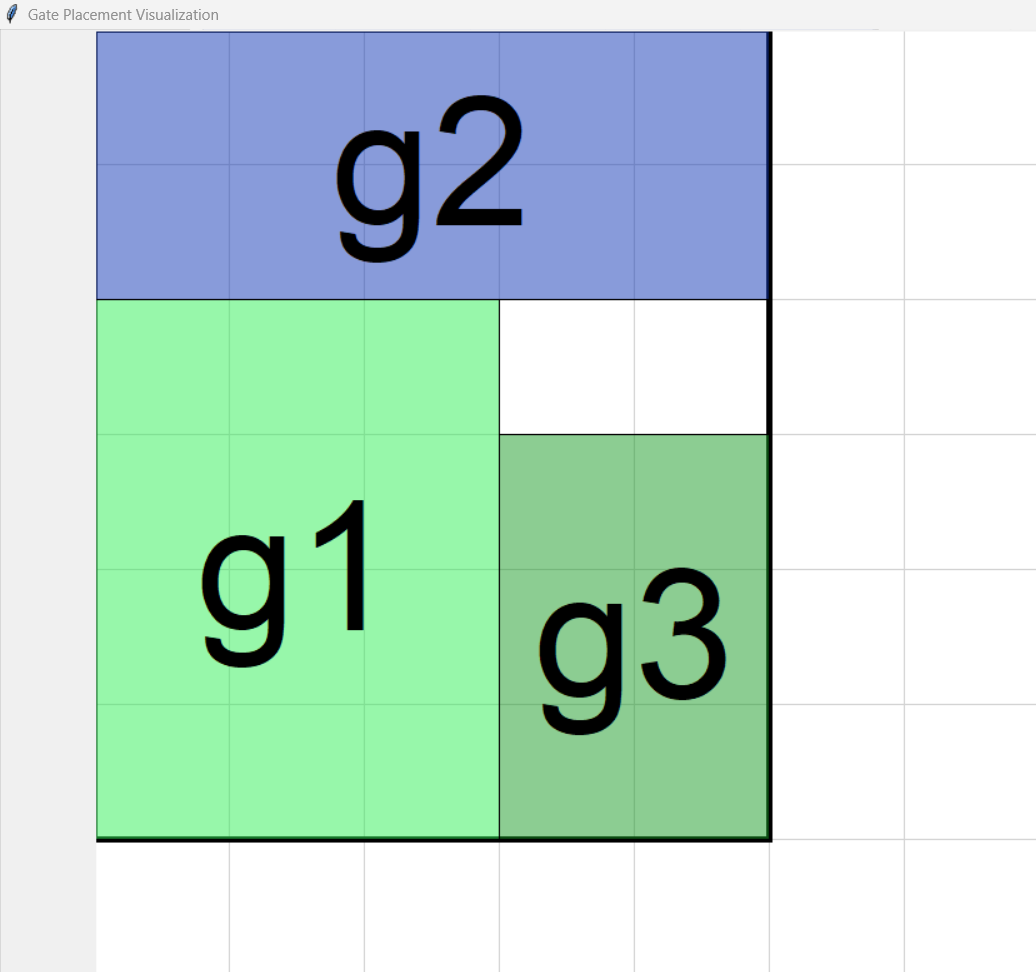
\includegraphics[width=1.0\linewidth]{Images/BRoll/Our_Packing_TC2.png}
          % \captionof{figure}{A figure}
          \label{fig:tc-2}
          \caption{Gate Packing }
     
          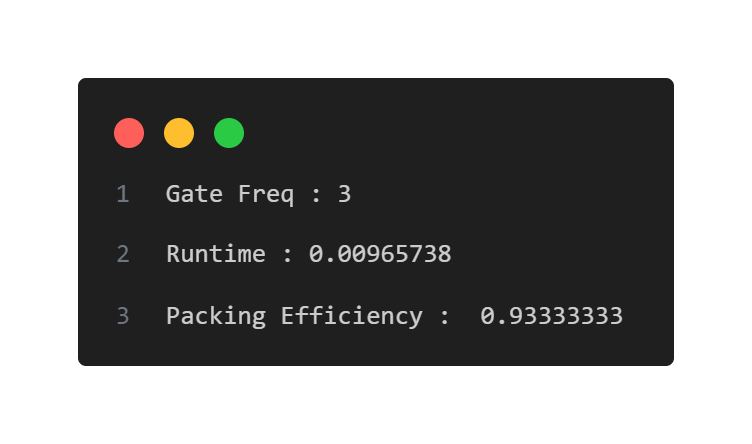
\includegraphics[width=0.95\linewidth]{Images/BRoll/Our_Packing_TC2_Report.png}
          % \captionof{figure}{A figure}
          \label{fig:tcr-2}
          \caption{Report}
    \end{minipage}
\end{figure}

    
\newpage
\subsection{Test Case 3}

\begin{center}
\begin{tabular}{|c|c|c|}
    \hline
    \rowcolor[HTML]{DAE8FC} Gate No. &
    Input \((w,h)\)                                    & Output \((x,y)\)  \\ \hline
    \rowcolor[HTML]{FFFC9E} {\color[HTML]{000000}\(1\)} &
    {\color[HTML]{000000} \((10,10)\)}                         & {\color[HTML]{000000} \((45,10)\)}    \\ \hline
    \rowcolor[HTML]{FFFC9E} 
    {\color[HTML]{000000} \(2\)} &
    {\color[HTML]{000000} \((20,5)\)}                         & {\color[HTML]{000000} \((35,25)\)}      \\ \hline
     \rowcolor[HTML]{FFFC9E} 
     {\color[HTML]{000000} \(3\)} &
    {\color[HTML]{000000} \((5,20)\)}                         & {\color[HTML]{000000} \((15,0)\)}      \\ \hline
    \rowcolor[HTML]{FFFC9E} {\color[HTML]{000000}\(4\)} &
    {\color[HTML]{000000} \((15,10)\)}                         & {\color[HTML]{000000} \((30,10)\)}    \\ \hline
    \rowcolor[HTML]{FFFC9E} 
    {\color[HTML]{000000} \(5\)} &
    {\color[HTML]{000000} \((10,15)\)}                         & {\color[HTML]{000000} \((20,0)\)}      \\ \hline
     \rowcolor[HTML]{FFFC9E} 
     {\color[HTML]{000000} \(6\)} &
    {\color[HTML]{000000} \((25,5)\)}                         & {\color[HTML]{000000} \((10,25)\)}      \\ \hline
    \rowcolor[HTML]{FFFC9E} {\color[HTML]{000000}\(7\)} &
    {\color[HTML]{000000} \((5,25)\)}                         & {\color[HTML]{000000} \((100,0)\)}    \\ \hline
    \rowcolor[HTML]{FFFC9E} 
    {\color[HTML]{000000} \(8\)} &
    {\color[HTML]{000000} \((30,10)\)}                         & {\color[HTML]{000000} \((30,0)\)}      \\ \hline
     \rowcolor[HTML]{FFFC9E} 
     {\color[HTML]{000000} \(9\)} &
    {\color[HTML]{000000} \((10,30)\)}                         & {\color[HTML]{000000} \((0,0\))}      \\ \hline
    \rowcolor[HTML]{FFFC9E} {\color[HTML]{000000}\(10\)} &
    {\color[HTML]{000000} \((35,5)\)}                         & {\color[HTML]{000000} \((15,20)\)}    \\ \hline
    
    
\end{tabular}
\end{center}
\begin{center}
\textbf{Bounding Box Dimension : Width = \(60\) , Height = \(30\)}     
\end{center}

\begin{figure}[ht]
    \centering
    \begin{minipage}{.6\textwidth}
          \centering
          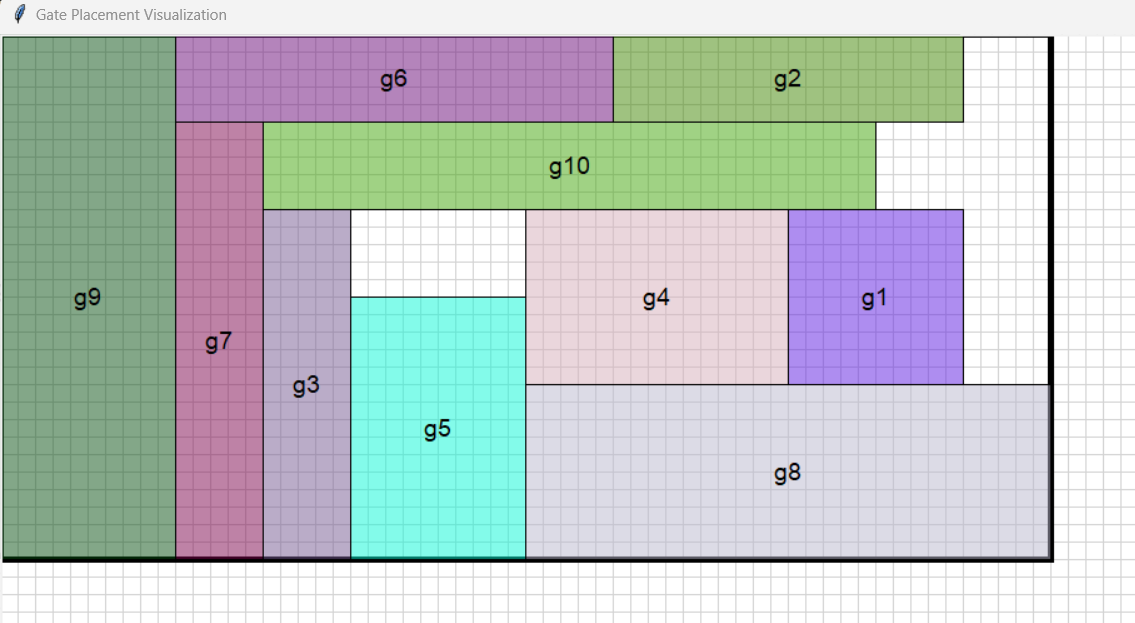
\includegraphics[width=1.0\linewidth]{Images/BRoll/Our_Packing_TC3.png}
          % \captionof{figure}{A figure}
          \label{fig:tc-3}
          \caption{Gate Packing }
      
          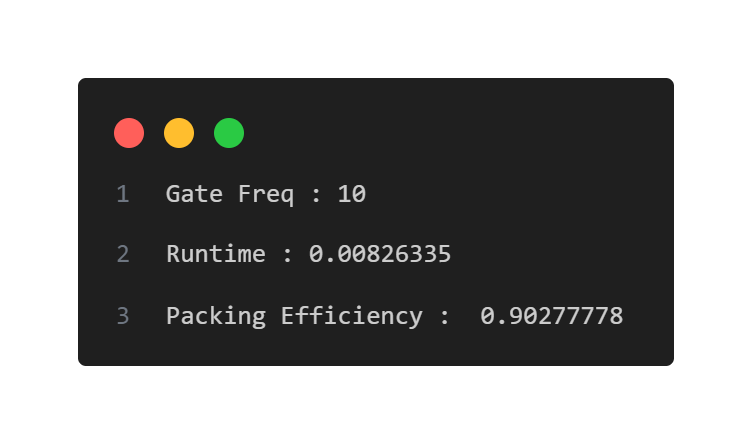
\includegraphics[width=0.95\linewidth]{Images/BRoll/Our_Packing_TC3_Report.png}
          % \captionof{figure}{A figure}
          \label{fig:tcr-3}
          \caption{Report}
          \centering 
      \end{minipage}
    \end{figure}

\newpage
\subsection{Test Case 4}
\begin{center}
\begin{tabular}{|c|c|c|}
    \hline
    \rowcolor[HTML]{DAE8FC} Gate No. &
    Input (w,h)                                    & Output(x,y)   \\ \hline
    \rowcolor[HTML]{FFFC9E} {\color[HTML]{000000}\(1\)} &
    {\color[HTML]{000000} \((4,5)\)}                         & {\color[HTML]{000000} \((2,0)\)}    \\ \hline
    \rowcolor[HTML]{FFFC9E} 
    {\color[HTML]{000000} \(2\)} &
    {\color[HTML]{000000} \((6,2\))}                         & {\color[HTML]{000000} \((6,4)\)}      \\ \hline
     \rowcolor[HTML]{FFFC9E} 
     {\color[HTML]{000000} \(3\)} &
    {\color[HTML]{000000} \((6,0)\)}                         & {\color[HTML]{000000} \((0,0)\)}      \\ \hline
      \rowcolor[HTML]{FFFC9E}  {\color[HTML]{000000}\(4\)} &
    {\color[HTML]{000000} \((3,4)\)}                         & {\color[HTML]{000000} \((6,0)\)}      \\ \hline
     \rowcolor[HTML]{FFFC9E} 
     {\color[HTML]{000000} \(5\)} &
    {\color[HTML]{000000} \((5,3)\)}                         & {\color[HTML]{000000} \((9,0)\)}      \\ \hline
    
    
\end{tabular}
\end{center}
\begin{center}
\textbf{Bounding Box Dimension : Width = \(14\) , Height = \(6\)} 
\end{center}

\begin{figure}[ht]
    \centering
    \begin{minipage}{.6\textwidth}
          \centering
          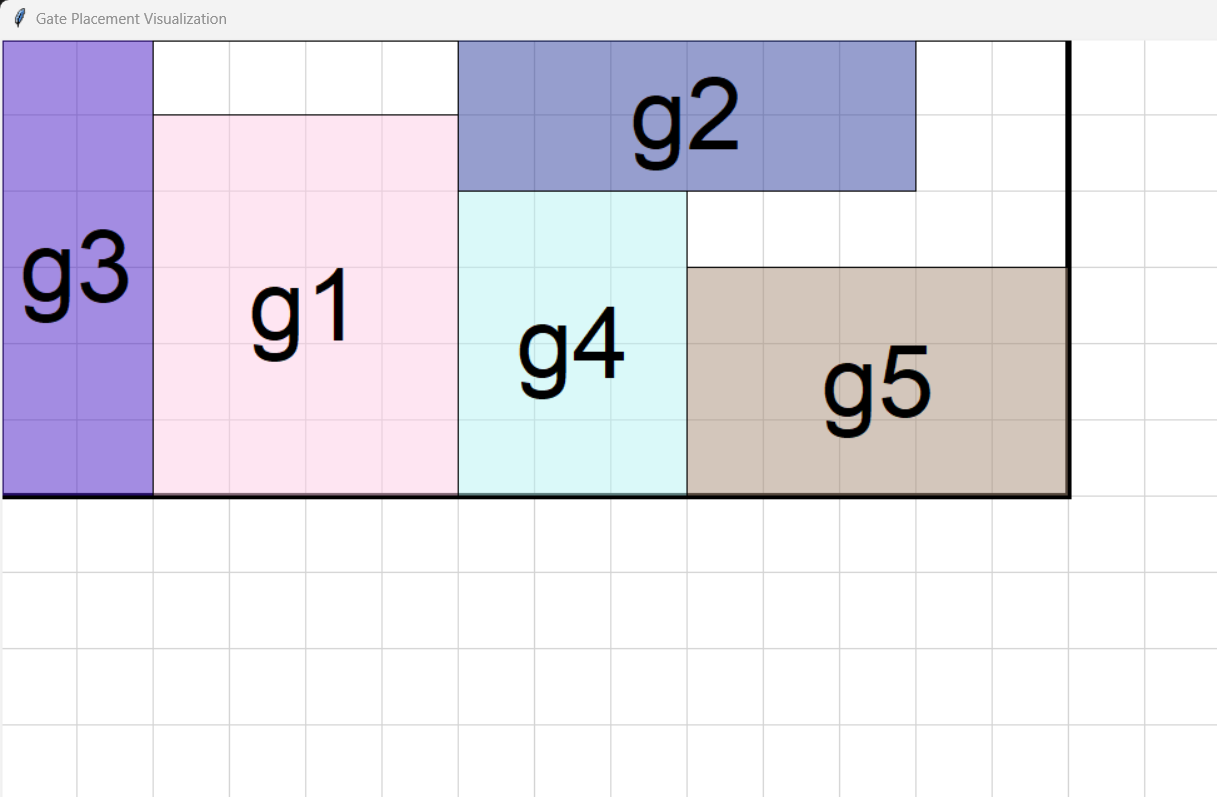
\includegraphics[width=1.0\linewidth]{Images/BRoll/Our_Packing_TC4.png}
          % \captionof{figure}{A figure}
          \label{fig:tc-4}
          \caption{Gate Packing }
     
          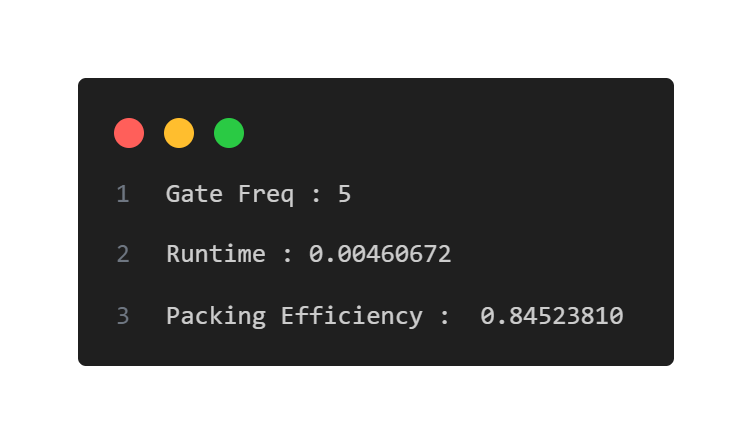
\includegraphics[width=0.95\linewidth]{Images/BRoll/Our_Packing_TC4_Report.png}
          % \captionof{figure}{A figure}
          \label{fig:tcr-4}
          \caption{Report}
          \centering 
      \end{minipage}
    \end{figure}

\newpage
\subsection{Test Case 5}
\begin{figure}[ht]
    \centering
    \begin{minipage}{.7\textwidth}
          \centering
          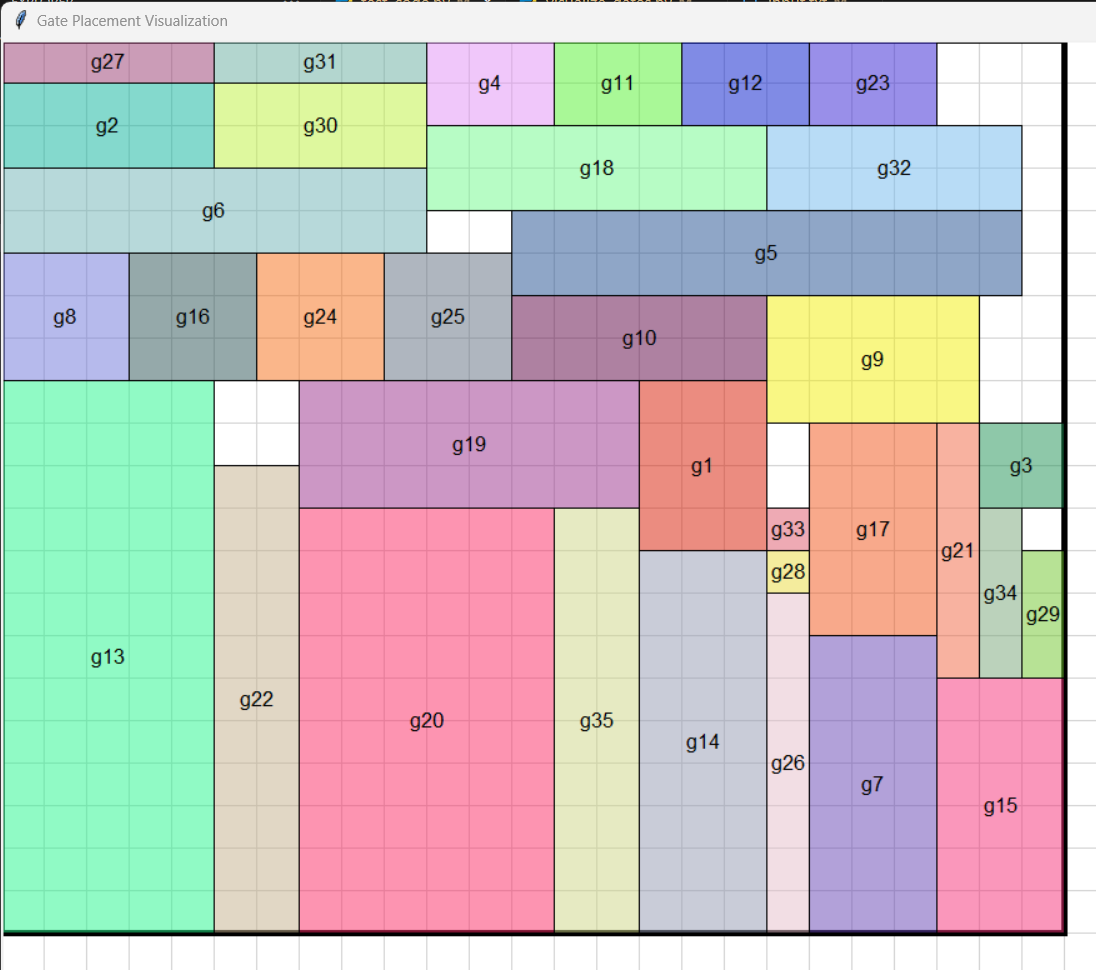
\includegraphics[width=1.0\linewidth]{Images/BRoll/output_sample_tc5.png}
          % \captionof{figure}{A figure}
          \label{fig:tc-5}
          \caption{Gate Packing }
      
          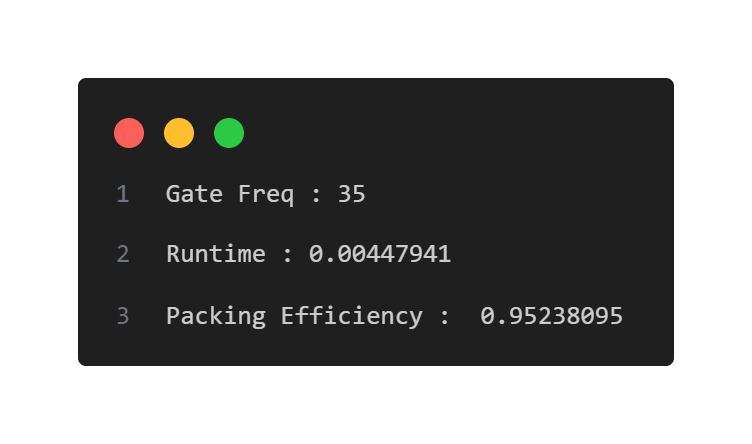
\includegraphics[width=0.95\linewidth]{Images/BRoll/Our_Packing_TC5_Report.png}
          % \captionof{figure}{A figure}
          \label{fig:tcr-5}
          \caption{Report}
          \centering 
      \end{minipage}
\end{figure}



\end{document}
%%%%%%%%%%%%%%%%%%%% End Of Document %%%%%%%%%%%%%%%%%%%%%%%%%%%
Document Authored by -
Yash Rawat - 2023CS50334  
Priyanshi Gupta - 2023CS10106 

%
 ___  ___  _________        ________         
|\  \|\  \|\___   ___\     |\   ___ \        
\ \  \ \  \|___ \  \_|     \ \  \_|\ \       
 \ \  \ \  \   \ \  \       \ \  \ \\ \      
  \ \  \ \  \   \ \  \       \ \  \_\\ \     
   \ \__\ \__\   \ \__\       \ \_______\    
    \|__|\|__|    \|__|        \|_______|    
                                             
                                             
                                             
 ________  ________  _______                 
|\   ____\|\   ____\|\  ___ \                
\ \  \___|\ \  \___|\ \   __/|               
 \ \  \    \ \_____  \ \  \_|/__             
  \ \  \____\|____|\  \ \  \_|\ \            
   \ \_______\____\_\  \ \_______\           
    \|_______|\_________\|_______|           
             \|_________|                                                           
%